\chapter{Credit Risk}

\section{Credit risk management}
Part of the daily business of a financial institution is the credit risk assessment of existing and new customers. The result will then be used to decide if they want to decline or grant a credit application and among other things, for setting the required regulatory capital. Credit risk assessment is performed during the whole lifetime of an exposure. It starts with the approval of a transaction and is continuously monitored afterwards. Corporate clients usually need to submit financial reports regularly, which is then analysed by their bank advisor and credit analyst, while for retail customers it is done automatically via behaviour scoring. The information used during the application scoring is limited because it is mainly provided by the applicant and generally covers variables about their financial health, e.g., income, outstanding debt. For the behaviour scoring model, internal historical data is used, for example the borrower's payment history and credit utilization. The behaviour model show a better predictive performance than the application model. If a decline of financial health or behaviour rating is detected, the bank may try to decrease the overdraft limit to regulate the credit risk. In the case of delayed payments, early collection process starts, where affected customers are contacted and an alternative payment plan will be negotiated. If all interventions fail, defaulted exposures may be sold or outsourced to collection companies for further processing like the sale of collateral. 

\section{Default Rate and Probability of Default}
\label{sec:dr_pd}
An important risk measure is the probability of default (PD), which is an estimate for the likelihood of a borrower failing to pay back their financial obligations in a given time period. Depending on the analysed portfolio, the expected number of defaults can vary. In the corporate segment, individual defaults can already be seen an indicator for a bank's failing credit assessment process and decision, while in the retail sector a higher number of default can be expected. In contrary, profit can be generated if the income gained from non-defaulted customers covers the loss from the defaulted portion of the portfolio.

\medskip
In the Capital Requirements Regulation (Capital Requirements Regulation, Article 178(1):), the definition of default is stated as:

\begin{quote}

A default shall be considered to have occurred with regard to a particular obligor when either or both of the following have taken place:
\begin{itemize}
\item[(a)] the institution considers that the obligor is unlikely to pay its credit obligations to the institution, the parent undertaking or any of its subsidiaries in full, without recourse by the institution to actions such as realising security;
\item[(b)] the obligor is more than 90 days past due on any material credit obligation to the institution, the parent undertaking or any of its subsidiaries. Competent authorities may replace the 90 days with 180 days for exposures secured by residential property or SME commercial immovable property in the retail exposure class, as well as exposures to public sector entities. The 180 days shall not apply for the purposes of point (m) Article 36(1) or Article 127.

\end{itemize}

In the case of retail exposures, institutions may apply the definition of default laid down in points (a) and (b) of the first subparagraph at the level of an individual credit facility rather than in relation to the total obligations of a borrower.

\end{quote}

A time period has to be defined in which a default event is observed. A common observation window is one year, a portrayal is visible in Fig. \ref{fig:cr_timeperiod}. The default rate per category (e.g., month, rating grade; given in Fig. \ref{fig:cr_defrate_year}. and \ref{fig:cr_defrate_ratgrade}.) is then calculated as the number of defaults divided by the total number of customers (Eq. \ref{eq:cr_dr}).

\begin{equation}
DR_{i} = \frac{d_{i}}{n_{i}} \label{eq:cr_dr}
\end{equation}
where:
\begin{conditions}
 d_{i}  & number of defaults in class i \\
 n_{i}  & number of observations in class i
\end{conditions}

\begin{figure}[H]
	\centering
	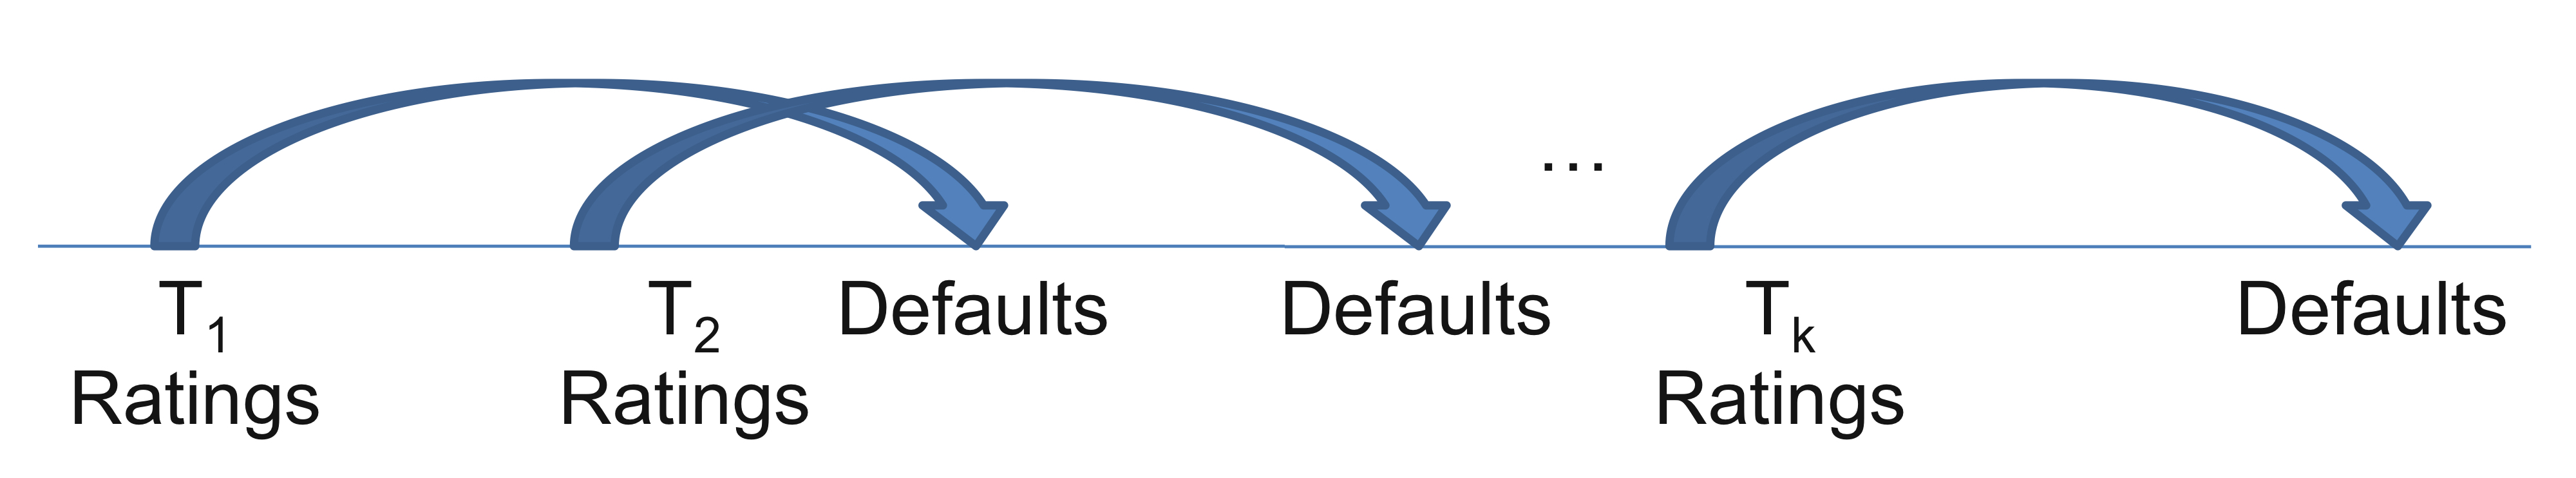
\includegraphics[width=.625\textwidth]{./CR__timeperiod.jpeg}
    \caption{Observation period after reference point}
    \label{fig:cr_timeperiod}
\end{figure}

\section{Regulatory Framework}

\subsection{History of regulatory framework}

The regulatory framework is set by the Basel Committee on Banking Supervision, which consists all regulators of the most developed countries. The goal is to define a high standard for risk management and internal controls, and establish a risk-sensitive calculation process of the regulatory capital for banks all over the world. The first Capital Accord was published in 1988 and since then was adapted and reformed numerous times. The New Capital Accord, also known as Basel II, was first issued in 2004 and underwent multiple amendments especially, after the financial crisis until July 2009. The European Union motivated the integration of these regulations by the Implementation Directive CAD 2006. In the end of 2010, a new reform called Basel III was  approved. 

\subsection{Credit risk regulatory capital}

The calculation of credit risk capital requirement was significantly improved compared to the first Capital Accord. Total loss of a bank can be split into expected and unexpected loss (Fig. \ref{fig:cr_elul}). The former should be covered by revenue and for the latter a bank is obligated to allocate an appropriate level of capital. The formula is given in Fig. \ref{fig:cr_capital_req} In the original approach, each exposure has been assigned into one of four risk categories and then a multiplier ranging 0-100\% was applied. Regulations now allow the Standardized (SA), Foundation or Advanced Internal Rating Based (IRBF, IRBA) Approach (Fig. \ref{fig:cr_reg_approaches}). In the SA five risk buckets are defined to calculate the regulatory capital and the Standard Approach also allows the use of external ratings. For the IRB, internal models estimate input parameters of the regulatory formulas, which then result in risk weights for each exposure. The IRBF approach only allows the estimation of the PD, while for the IRBA the risk parameters Loss Given Default, Exposure at Default, Conversion Factor and Effective Maturity are additionally derived from internal models. The corporate segment permit both IRBF and IRBA approaches, but for the retail portfolio, only the IRBA is possible.

\begin{figure}[H]
	\centering
	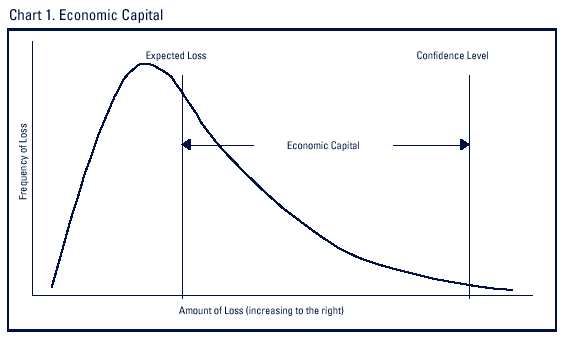
\includegraphics[width=.625\textwidth]{./CR__EL_UL_capital.png}
    \caption{Economical Capital, Expected and Unexpected Losses}
    \label{fig:cr_elul}
\end{figure}

\subsection{Challenges and Limitations}

Good data is of utmost importance for the credit risk assessment. While it will be used for modelling purposes, it is also important that already known negative information of customers is available  and taken into consideration. Examples are internal information, for example a client already has a history of fraudulent activity during a credit application, or credit bureau information, where negative credit information is made available for all participants. In Austria, institutions are Kreditschutzverband (KSV) and CRIF. 

Other possible challenges are the constant change in economic conditions and regulatory frameworks, which have an influence on the PD estimates. In addition, during the PD estimation the default event of individual borrowers are assumed to be independent, which does not adequately capture behavioural risks (e.g., strategic default) or systemic risks (e.g., market-wide shocks) that can affect multiple borrowers simultaneously. It is therefore important that PD models are continuously refined and adapted to accurately reflect current economic situation.